\section{Benchmarking}
Throughout the project we had two goals in mind in terms of performance:
\begin{enumerate}
    \item Calculate the $\mathbf{A}$ matrix faster than the reference python solution provided 
    by Associate Professor François Lauze.
    \item Calculate the $\mathbf{A}$ matrix faster than, or comparable to, reading the matrix from disk.
\end{enumerate}
To answer whether we have achieved these goals or not, we utilize the build-in 
benchmarking suite provided by Futhark. 

\subsection{Against Reference Solution}
A reference solution implemented in python was provided by François Lauze. 
Due to CPUs and GPUs being fundamentally different devices, it is difficult to strongly argue which two devices to use for comparison. We ran the sequential python code on an Intel i7-4790K 4.40GHz processor and the parallel Futhark code on a Nvidia 780ti GPU with 3GB of VRAM, since these two devices were released at roughly the same time, and both were similar high end consumer products on their respective markets.

As a preliminary comparison, we tested the two solutions with the following parameters:
\begin{table}[H]
    \centering
    \label{phantom}
    \begin{tabular}{ll}
        Grid size & 2000 \\
        Lines     & 2000 \\
        Angles    & 15 
    \end{tabular}
    \caption{Reference Parameters}
\end{table}
From table \ref{fig:phantom_results} we notice a significant speed difference between the two solutions, with the GPU-based Futhark implementation coming in at 0.03 seconds, while the CPU-based python implementation takes almost 10 seconds. We thus beat the reference solution with a factor of 300. 
\begin{table}[H]
    \centering
    \begin{tabular}{llll}
        Implementation   & Hardware & Microseconds & Seconds \\
        \hline
        Futhark (OpenCL) & GTX 780ti - 2880 cores @ 928MHz    &34155.20      & 0.03    \\
        Python           & Intel i7-4790K @ 4.40GHz    &9430491      & 9.43     
    \end{tabular}
    \caption{Reference Parameter Benchmarking Results}
    \label{fig:phantom_results}
\end{table}
While the above results are positive, we are of course interested in seeing how well each solution scales with problems of different sizes, and if this scaling depends on which parameter is being changed.
For this purpose, we compiled a CPU-based C version of our Futhark code, and compared this to our regular GPU-based OpenCL version. For practical reasons, it was necessary to switch out the i7-4790K with a Xeon E5-2650 processor, noting that the E5-2650 is significantly slower than the i7-4790K, but we deemed this to not be a problem, unless we saw similar execution times between the GPU and CPU solutions, in which case a faster CPU might have tipped the comparison in favour of the CPU.
\begin{table}[H]
    \centering
    \label{opencl_v_c}
    \begin{tabular}{ll}
        Implementation   & Hardware  \\
        \hline
        Futhark (OpenCL) & GTX 780ti - 2880 cores @ 928MHz      \\
        Futhark (C)      & Intel Xeon E5-2650 @ 2.60GHz     
    \end{tabular}
    \caption{Hardware for Futhark-OpenCl vs Futhark-C}
\end{table}
If we begin by letting the grid size vary, we notice that the GPU and CPU versions take almost the same amount of time for small grids of $200$, but as the grid size grows, the GPU version significantly outperforms the CPU version. It is apparent, that while both versions exhibit linear time complexity, they grow at very different rates, and as such, the GPU version only needs around $35$ms to calculate the line intersection of a $3000\text{x}3000$ grid, while the CPU requires around $1250$ms. There is thus a factor of $35$ between the two solutions, and this factor increases as the grid size grows larger. 
\begin{figure}[H]
    \centering
    \captionsetup{justification=centering,margin=2cm}
    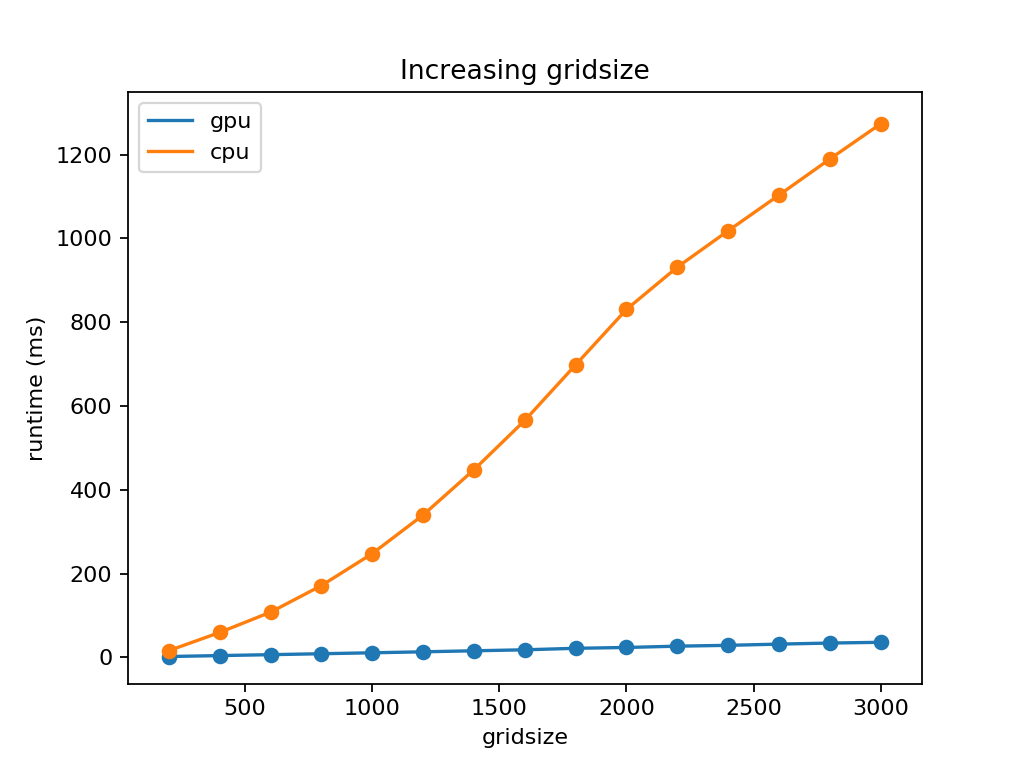
\includegraphics[scale=0.6]{figures/gridsizeGPU_gridsizeCPU.png}
    \caption[caption]{Running times with increasing grid size\\\hspace{\textwidth}2000 lines, 10 angles}
\end{figure}
To some extend, the result above is surprising, seeing that the increased grid size is not parallelized, since the grid intersections of each line is solved sequentially. However if we remember that the test is performed on $2000$ lines and $10$ angles, it is clear that there is a fair degree of parallelization in the test scenario, explaining the good performance of the GPU solution, even for small grids. This does however indicate, that there is a minimum degree of parallelization needed, before the GPU solution becomes faster than the CPU, and this cutout appears to be around $20000$ concurrent parallelized tasks, since we see the CPU and GPU performing equally well at a line count of $2000$ over $10$ angles.

Moving on to increasing line counts, we see a similar pattern as with increasing grid size. As the line count increases, the running times of each solution diverges, reaching $400$ms for the CPU solution, and $35$ms for the GPU solution, when the line count is $3000$. We notice two odd jumps in the CPU's runtime on line counts of $200$, $400$ and $600$, followed by a linear development from that point on. These jumps are ascribed to the CPU running out cache, requiring utilization of ever slower cache/memory.
\begin{figure}[H]
    \centering
    \captionsetup{justification=centering,margin=2cm}
    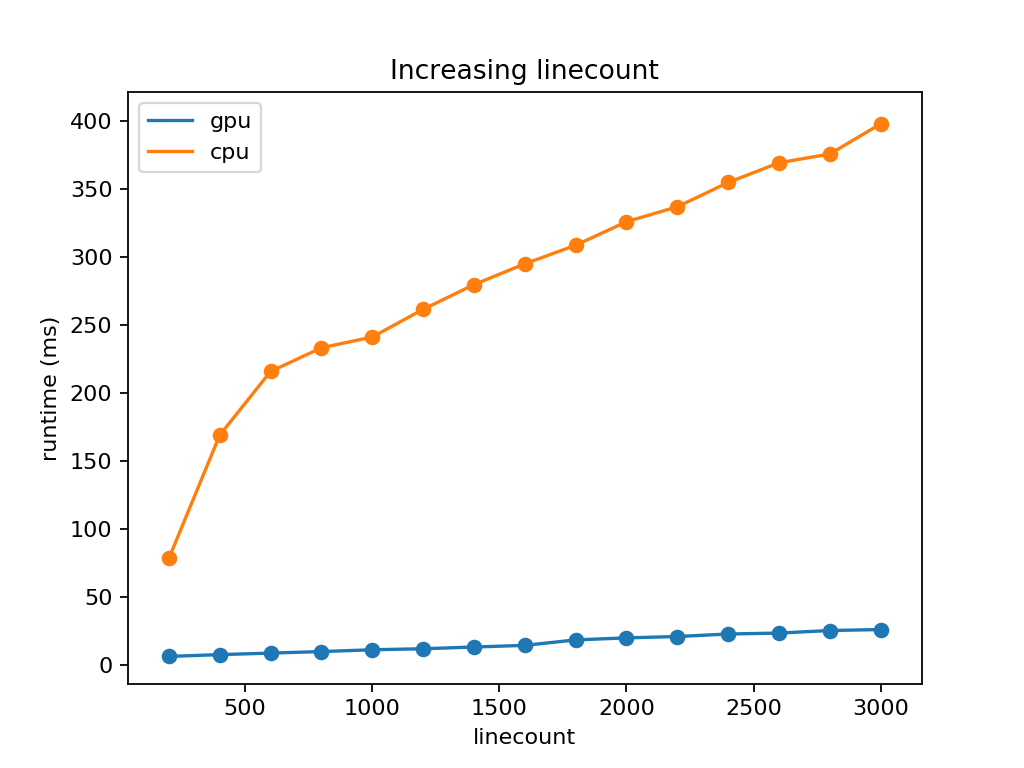
\includegraphics[scale=0.6]{figures/linecountGPU_linecountCPU.png}
    \caption{Running times with increasing line count\\\hspace{\textwidth}2000 grid size, 10 angles}
\end{figure}
Figure \ref{bench_angles} shows the running times associated with an increasing amount of angles. Both solutions show linear developments, but with very different slopes. Once again we see the GPU outperforming the CPU, with the gap growing larger, as the number of angles increase. The GPU solution requires $18$ms to calculate the grids for $30$ different angles, while the CPU needs $700$ms to solve for the same amount of angles. 
\begin{figure}[H]
    \centering
    \captionsetup{justification=centering,margin=2cm}
    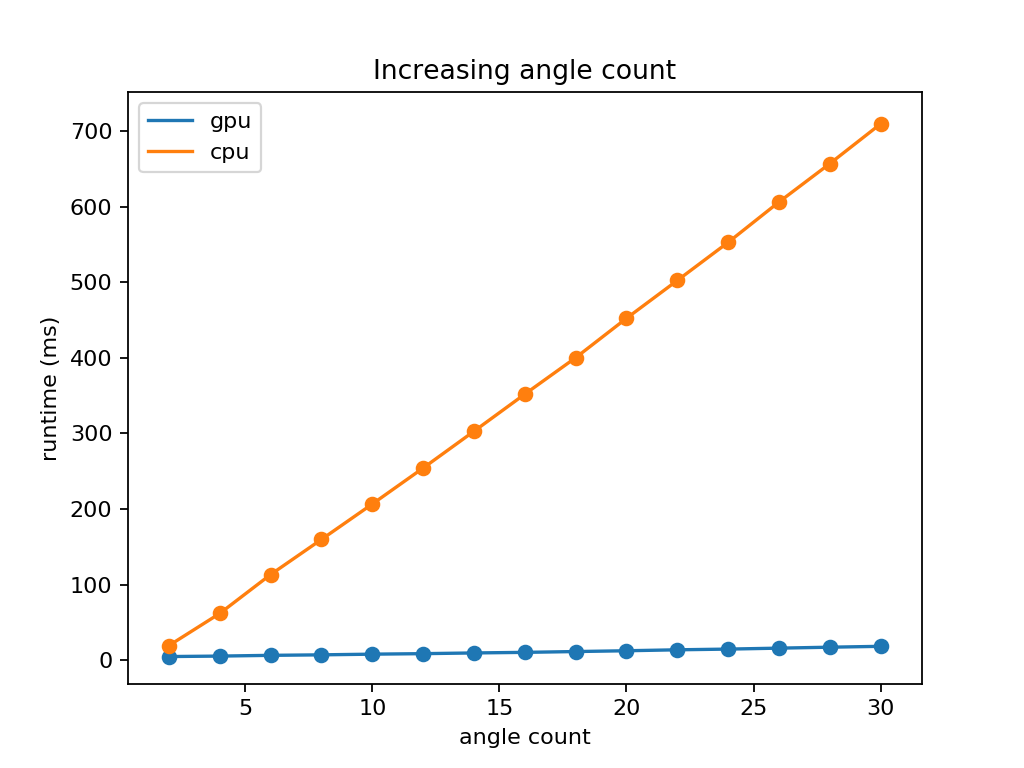
\includegraphics[scale=0.6]{figures/anglesGPU_anglesCPU.png}
    \caption{Running times with increasing number of angles\\\hspace{\textwidth}1000 grid size, 500 lines}\label{bench_angles}
\end{figure}
Overall, it must be concluded that the GPU solution significantly outperforms the CPU solution, even for relatively small problem sizes, such as the ones we tested on. 

\subsection{Against Reading From Disc}
Testing against a modern SSD with a SATA 3.0 6Gb/S interface, we found the GPU solution to be roughly 10 times faster, although with some uncertainty and variability. The tests were performed by saving grid intersection data as binary files, and then reading the system time before and after reading from the files in a \texttt{C}-program. To mitigate the problem, that the system could schedule unrelated tasks within this time interval, we averaged over 10 samples for each data point. This also warms up the cache, bringing down the average runtime, but since this cache effect is \textit{not} in favor of our GPU solution, we deemed this not to be a problem for the validity of our conclusion. As shown on figure \ref{fig:disk}, even though reading from the SSD is fast, it is not fast enough to overcome the calculation speed of the GPU. We see that for a line count of $2000$ the Futhark codes uses $25$ms to solve the problem, while reading from disk takes $350$ms. The benchmark of the Futhark code excludes the cost of transferring the  data from GPU to main memory, but since a modern PCIE slot with 16 lanes has a transfer rate of 31.51 GB/s, and the data size corresponding to $2000$ lines being $590$MB, the cost of transferring the data should in theory only be around $150$ms\cite{PCIE}. Thus recalculating the data should still be faster, although less so. 
\begin{figure}[H]
    \centering
    \captionsetup{justification=centering,margin=2cm}
    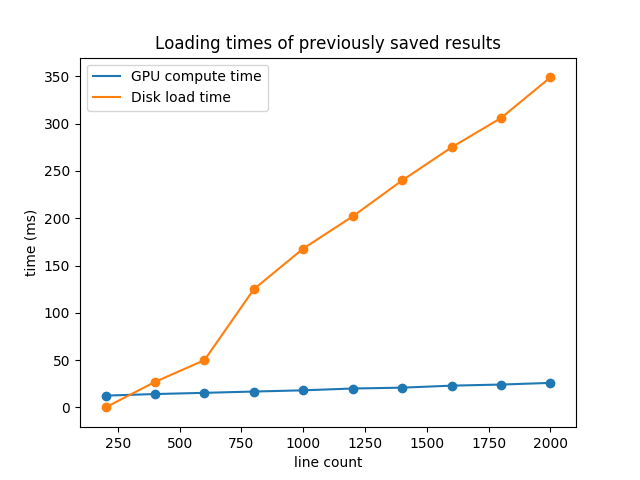
\includegraphics[scale=0.6]{figures/loadtime.png}
    \caption{Reading from disk vs. recalculating}\label{fig:disk}
\end{figure}
While reading from disk may still be an attractive option, in situations where a high performance GPU is not available, our benchmarking suggests that on-the-fly calculations are not only feasible, but in fact faster than reading from disk. 

\iffalse
Intel SSD 520 Series
240GB, 2.5in SATA 6Gb/
\fi